\chapter[Explicit predictive current control]{Explicit model predictive control of a current source buck-type rectifier}\label{BASIC:sec:MPC_CSR}

\section{Literature overview}\label{BASICCSR:sec:CSR_Literature}

%============ USAGE OF CURRENT SOURCE RECTIFIERS
Current source rectifiers (CSR) are widely used in front-end power electronic converter for the uncontrollable or controllable DC-bus in industrial and commercial applications. They have maintained their position through many applications, with uses such as medium-voltage high-power drives \cite{vajda2017limiting}, \cite{ghalem2010six} STATCOMs \cite{gupta2014two} and renewable systems \cite{chen2016single}, \cite{exposto2015predictive}. They have a plain and reliable circuit structure, which makes them attractive for simple control design. The CSRs are traditionally controlled by state feedback, or classic cascaded linear control loops such as PI controllers. These simple control applications are suitable for induction motor control \cite{chebre2011speed}, and other electromechanical actuators \cite{salloum2014robust}, and unusual topologies \cite{neukirchner2017voltage}. Also, worth mentioning of self-tuning variants of PI controllers \cite{tahri2012digital}.\\
%============ MODULATION OF CSR
 In the past, the modulation methods used were trapezoidal pulse width modulation techniques (TPWM), or application of pulse patterns calculated off-line for selective harmonic elimination (SHE). More recently, current space vector modulation (SVM) has been used for the synthesis of the transistor control signals \cite{gao2017model}. Even so, AC-side harmonic elimination could still be an issue at lower switching frequencies where LCL filtering (inductive-capacitive-inductive) would be advised \cite{han2010control}.\\
%============ TOPOLOGIES OF CSR
%In order to keep switching frequencies low and to minimize switching losses, new topologies and hybrid modulations are used, mixing TPWM and SHE depending on the grid frequency \cite{venkatraman2018multilevel}.\\
%============ BENEFITS OF CSR
    In terms of the amplitude of the grid and DC-link voltages, CSRs exhibit a step-down conversion. When used as DC voltage source, the rectifier can output a lower DC voltage without the need of a grid-side transformer, as is usually employed in voltage source rectifiers (VSR). Because of their current source behavior, CSRs can easily be paralleled and provide inherent short-circuit protection, representing an excellent potential in DC power supply applications \cite{feroura2017finite}, \cite{yan2015study}.\\		
%============ GENERAL CSR CONTROL
    %General
    There are several control strategies in addition to classical PI control for applications in this domain. Self-adapting control methods are on the rise with more sophisticated algorithms, although with varying degree. \hlc[PT]{Filtering the AC side of three-phase current source PWM rectifier is realised with LC filtering, bringing leading power factor and oscillatory current to the set of solvable problems. This means, beside the neccesary power factor correction, by ofsetting the equation set's quadratic component based on further active components and loads, the LC filter acts as a general low pass filter for the high frequency transitions but brings oscillations into the system's dynamics, which need to be compensated. Over sizing this LC filter or the choke inductance (which smoothes the DC current) makes the design not only more expensive to build, but load dynamics could be dampened, making it insufficient for drive control. On top of that, the bilinear nature of PWM rectifier's equation set, makes it difficult for designing control. This means, the sufficient effect could not be obtained with the traditional PID control system under larger disturbance and changes of controlled object, in other words, the general approach suffers from dynamic problems.}\\
    %Adaptive state feedback
    \hlc[PT]{The resonance can come either form the PWM process or from the grid voltage distortions, hence results in line current distortion. In }\cite{bai2013resonance}\hlc[PT]{ state feedback controllers were analysed using different variables in the filtering process. It is shown by }\cite{wiseman2005active}\hlc[PT]{ that  the  inductor-voltage  feedback  or  the  capacitor-voltage feedback can damp the current oscillations by increasing the damping ratio. The results show that voltage feedback can effectively damp the current oscillations but are unable to suppress the low-order harmonics from low frequency switching. On the other hand, the current feedback can contribute to the  suppression of the low-order harmonics but the damping ratio cannot be increased. However, the combined variable feedback controls, can achieve both results.}\\
    %Fuzzy
    \hlc[PT]{The author of} \cite{zheng2010current}\hlc[PT]{ is proposing the combination traditional PID control with fuzzy control, for a current source rectifier setup based on fuzzy two closed loop control system. The analysis of the differential equations proved, a decoupling is possible for two independent closed loop self-adaptive fuzzy control strategy with disturbance and oscillation compensation. Despite the hardships of tuning a fuzzy controller, good robustness is realized, with of fuzzy controller making the system's interferences to damp and eliminating the time variance.}\\
    %
    With model augmentation it is possible to handle increasingly more complicated models and systems with high dynamics and accuracy \cite{chatterjee2008augmented}, \cite{haidegger2012simulation}, and even without establishing and validating classical state-space models \cite{vrkalovic2018model}. The other filed is the sliding mode control, which can achieve good dynamic performance and handle non-linearity. Still, they might also introduce chattering, which can be very undesirable when applied to real-life systems like in \cite{regaya2014new} and \cite{szell2014mathematical}. Additionally in \cite{ahmed2014model} the validity of an MPC-based, digital pulse width modulation control strategy for single-phase voltage source rectifiers is discussed, further confirming the validity of this method in control systems.\\
%============ PREDICTIVE POWER ELECTRIC CONTROL	
    %Basic
    \hlc[PT]{A a basic premise a simple predictive control scheme for CSRs is presented in} \cite{correa2008predictive}, \hlc[PT]{where the control scheme considers the discrete change of   switching states at equidistant points with a constant sampling period. The measured output current follows the reference current very closely even under transient  conditions,which corroborates the good dynamics provided with the proposal. This makes the model based predictive controller so popular, since control design is much more straightforward and systematic, if the boundary conditions, like linear system design, or perfectly known system model and load can be achieved. However, this is also a requirement of other control schemes based on PID controllers and modulators. As a further step adaptive application was established to tackle parameter estimation problems for better performance in uncertain modeling situations} \cite{muthukumar2016adaptive}.\\
    %Advanced	
    In the linear domain implicit model predictive control (IMPC or MPC) is the next evolutionary step due its effectiveness because of its configurable cost function and such scalable nature \cite{kelemen2010constrained}, \cite{ahmed2014model}. \hlc[PT]{In this state, variable step size for computation benefits or refined local control dynamics is also an option.} In this field also finite-state solutions are present which can be considered also predictive control, where the modulation scheme’s defined states serve as optimization potential \cite{rivera2013predictive}, \cite{godlewska2015predictive}. \\	
%============ EXPLICIT PREDICTIVE CONTROL
    Recently, beside implicit, finite-state, and adaptive predictive control, explicit model predictive control has emerged in the field of power electronics \cite{kutasi2010constrained}. Establishing the MPC cost function can range widely depending on the expected dynamics, degree of noise cancellation, and model complexity. \hlc[PT]{Additionally, embedded state- or input constraints can also be implemented introducing constraints in the control algorithm. This is very beneficial in safety, or automotive applications. However the main advantage, is the the significant reduction of calculation demand, enabling for much higher switching frequencies in applications. This enables the designer to choose lower LC values making the damping design also easier.}\\	

\section{Three-phase buck-type rectifiers}\label{BASICCSR:sec:CSR}

Three-phase controlled rectifiers have a wide range of applications, from small rectifiers to large high-voltage direct-current transmission systems. They are used e.g. at electrochemical processes, many kinds of motor drives, traction equipment, controlled power supplies. In this thesis only force commuted rectifiers are examined, which are built with semiconductors (IGBTs in this case) with gate-turn-off capability. The gate-turn-off capability allows full control of the converter, because valves can be switched ON and OFF whenever is required. This allows the commutation of the valves, hundreds of times in one period that is not possible with line-commutated rectifiers, where IGBTs are switched ON and OFF only once a cycle. This has the following advantages:

\begin{itemize}
\item The current or voltage can be (pulse width) modulated, generating less harmonic contamination.
\item The power factor (ratio of the real and reactive power) can be controlled and even it can be made leading, signifies that the load is capacitive, as the load “supplies” reactive power.
\item They can be built as voltage-source or current-source based on the required application.
\item The reversal of power in switching rectifiers is by reversal of voltage at the DC link. This allows force commutated rectifiers can be implemented for both, reversal of voltage or reversal of current.
\end{itemize}

There are two ways to implement force commutated three phase rectifiers, as a current-source rectifier (Fig.\ref{BASICMPC:fig:CSR}), where power reversal is by DC voltage reversal, and as a voltage-source rectifier (Fig.\ref{BASICMPC:fig:VSR}), where power reversal is is solved by current reversal at the DC link.


\begin{figure}[h]
                \centering
                \begin{subfigure}[b]{0.9\textwidth}
                    \includegraphics[width=\textwidth]{EMPC_PNG_Pics/BasicCurrentRectifiers.png}
                    \caption{\centering Current source rectifier with capacitive filtering and choke inductance.}
                    \label{BASICMPC:fig:CSR}
                \end{subfigure}
                ~ %add desired spacing between images, e. g. ~, \quad, \qquad, \hfill etc.
                  %(or a blank line to force the subfigure onto a new line)
                \begin{subfigure}[b]{0.9\textwidth}
                    \includegraphics[width=\textwidth]{EMPC_PNG_Pics/BasicVoltageRectifiers.png}
                    \caption{\centering Voltage source rectifier with inductive filtering and DC voltage smoothing capacitance.}
                    \label{BASICMPC:fig:VSR}
                \end{subfigure}
                 %add desired spacing between images, e. g. ~, \quad, \qquad, \hfill etc.
                %(or a blank line to force the subfigure onto a new line)
                %\begin{subfigure}[b]{0.48\textwidth}
                    %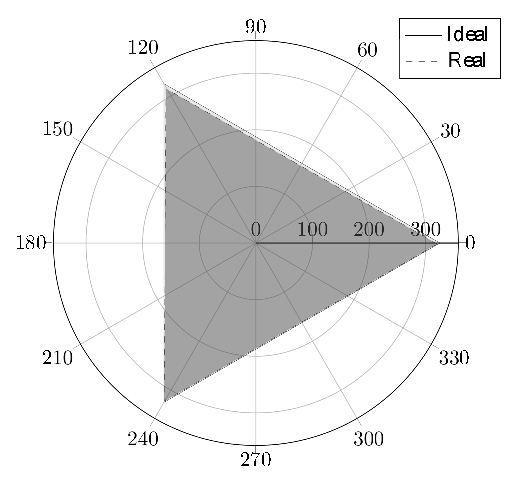
\includegraphics[width=\textwidth]{Unblance_EPS_Pics/EPS_images/square.eps}
                    %\caption{Low correlation with opposed amplitude deviation. The norm values are $G=9322$ and $TDV=0.5198$.}
                    %\label{fig:cases_C}
                %\end{subfigure}
                %~
                %\begin{subfigure}[b]{0.48\textwidth}
                    %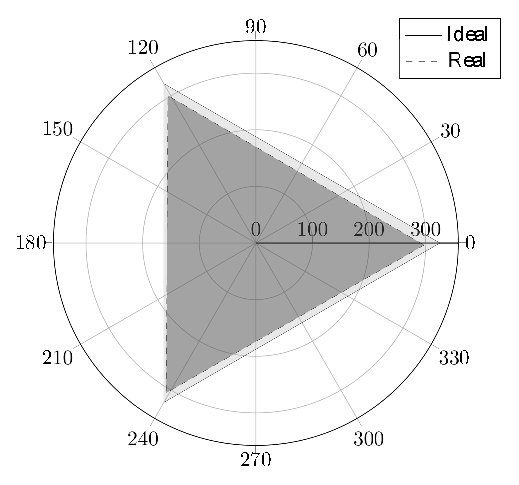
\includegraphics[width=\textwidth]{Unblance_EPS_Pics/EPS_images/circle.eps}
                    %\caption{\centering Low correlation with uniform voltage drop. The norm values are $G=6280$ and $TDV=0.156$.}
                    %\label{fig:cases_D}
                %\end{subfigure}


                \caption{Basic topologies of force commuted rectifiers.}
            \end{figure}

%\begin{figure}[!ht]
        %\centering
        %\includegraphics[width=0.9\textwidth]{EMPC_PNG_Pics/CurrentVoltageRectifiers.png}
        %\caption{Basic topologies of force commuted rectifiers.}
        %\label{BASICCSR:fig:topologies}
    %\end{figure}


As  general case be a front-end  converter power supply (e.g. lighting or telecommunications) shall be designed such that it should have approximately these general characteristics: sinusoidal main currents, unity power factor, high power density and simplicity of the power circuit structure. Two structures are most fitted for the task. First a boost-type input rectifier (e.g., Vienna rectifier, \cite{kolar1996design}), that typically features two $400$ V output voltages with a three-level isolated  DC-DC  converter  or  two  isolated  DC-DC  output  stage (see Fig. \ref{EMPC:fig:network} in Ch.5.). The second candidate is the buck-type  input  rectifier (or current source rectifier (CSR))  (conventionally  six-switch topologies as proposed in \cite{zargari1993current}, \cite{sato1993state}) with only one two-level isolated  DC-DC  converter  output  stage.  Also the  input  stage  can be realized as a three-switch topology with considerably  lower  system  complexity  as  compared  to  the boost-type structure. In particular, the number of utilized active and passive components is much lower. Furthermore, there is no middle-point that has to be stabilized, as this is the case for the boost-type structures, making control and active filter design less complex. Further system advantages are the potential of direct start-up and the implicit over current protection in case of an output short circuit. Therefore, these topologies of high interest for many safety critical applications as such future electric aircraft, or automotive applications or as power supplies for process technology \cite{nussbaumer2007comprehensive}.
The three-switch buck rectifier topology was first proposed in \cite{malesani1987three}. In \cite{itoh1989steady} and \cite{tooth2000effects}, aspects of the system modulation and control have been treated. The application of the topology used as an active filter is discussed in \cite{salo2005three}.  The addition of a DC-DC output boost-stage has been proposed in \cite{baumannnew} in order to maintain 400 V output voltage for a wide input voltage range and for the case of unbalanced mains as, e.g., the loss of one phase.

\myparagraph{Basic operation principles}\label{BASICCSR:sec:OperationPrinciple}

For the derivation of the relative on-times of the three buck transistors $S_i$ with the following assumptions are made for clarity and facilitation of calculations:
\begin{itemize}
	\item The AC-side filter capacitor voltages ($v_{c_p}$, where $p\in\{1,2,3\}$) at the input of the CSR are sinusoidal and in phase with the main harmonic component of voltage.
	
	\begin{equation}
        \begin{array}{rcl}
            v_{c_1}&=&\widehat{v}_c\cos(\omega t)\\
						v_{c_2}&=&\widehat{v}_c\cos(\omega t-2\pi/3)\\
						v_{c_3}&=&\widehat{v}_c\cos(\omega t+2\pi/3),\\
        \end{array}
        \label{BASICMPC:equ:phasorvect}
    \end{equation}
	where $\omega$ is the network voltage's angular velocity.
	
	\item The mains currents are assumed to be equal to the fundamental component of the rectifier input currents.
	\item The current in the DC output inductor $L_{D}$ is not affected by the high frequency ripple due to the switching operation.
\end{itemize}

 For achieving ohmic mains behavior also in case of unbalanced fundamental harmonics conditions the explained modulation method can still be utilized, however, additionally the control structure presented in \cite{baumann2005novel} has to be employed.\\
The waveforms of the phase and line-to-line mains voltages are divided into twelve sectors of $\frac{\pi}{6}$ rad wide shown in Fig.\ref{BASICCSR:fig:waves}. The following calculations are based on the analysis of the first sector which is characterized by the voltage harmonic phase relation. For the remaining sectors the calculations can be accomplished in an similar manner \cite{nussbaumer2007comprehensive}.

\begin{figure}[!ht]
        \centering
        \includegraphics[width=\textwidth]{EMPC_PNG_Pics/Waves.png}
        \caption{Phase voltages $v_{i}$, where line-to-line voltages $v_{N,ij}=v_{N,i}-v_{N,j}$, $(i,j)\in\{R,S,T\}$ and sectors $1$ to $12$ being defined by the different relations of the instantaneous values of the mains phase voltages for $v = 400 V$}
        \label{BASICCSR:fig:waves}
    \end{figure}
		
		Accordingly, on AC side, if conditions are favorable, inductor current can appear in an instant of time either in two out
of three phases or in none. In this modulation technique, the switches in each converter leg can conduct only one at the time (aside from zero states, where both upper and lower switches are conducting). When the upper leg is conducting it is indicated by `$1$', when the lower  `$-1$' and when neither `$0$'. As such the choice whether upper or lower switch of the leg conducts current depends of the reference current vector's sector location.
According to the actual switch combination the DC link current shaped by the choke inductance, and distributed to two of the input phases or the freewheeling diode. With this, the input current space vectors can be calculated for each of the before-mentioned switching states. Generally the space vector of three-phase quantities (e.g., for the rectifier input current) are described as:

\begin{equation}
        \begin{array}{rcl}
            \vec{i}&=&\frac{2}{3}\left(\vec{i}_a+\vec{i}_be^{\frac{j\pi}{3}}+\vec{i}_bc^{\frac{4j\pi}{3}}\right).\\
        \end{array}
        \label{BASICCSR:eqn:currents_all}
    \end{equation}
		
		Based on \ref{BASICCSR:eqn:currents_all} the corresponding active space vectors in the first sector can be obtained as:
		
		\begin{equation}
        \begin{array}{rcl}
            \vec{i}_{(1,0,-1)}=\vec{i}_1&=&2i_{dc}e^{j\pi/6}/\sqrt{3}\\
						\vec{i}_{(0,1,-1)}=\vec{i}_2&=&2i_{dc}e^{j\pi/2}/\sqrt{3}\\
						\vec{i}_{(-1,1,0)}=\vec{i}_3&=&2i_{dc}e^{j5\pi/6}/\sqrt{3}\\
        \end{array}
        \label{BASICCSR:eqn:currents}
    \end{equation}
		
		The resulting discrete space vectors can be used to synthesize desired current
space vector $\vec{i}_{ref}$.

The modulation methods were evaluated in and chosen for this paper based on \cite{moussaoui2005open}, which ensures minimum switching-losses, minimum ripple values of the input capacitor voltages and of the output inductor current. According to this modulation, each pulse interval comprises two active states and a freewheeling state, arranged symmetrically about the middle of the pulse interval (see Table \ref{EMPC:tbl:sequence}). For more in depth functional description see section \ref{EMPC:sec:Modulation}.

\subsection{Coordinate transformations}

In section \ref{EMPC:sec:ModelofCSR} the three phase current source rectifier's (CSR) equations are converted to different coordinate spaces.

\subsubsection{Clarke transformation}\label{BASICCSR:sec:Clarke}

In electrical engineering, Clarke transformation is a mathematical transformation employed to simplify the analysis of three-phase circuits. Conceptually it is similar to the Park transformation. One very useful application is the generation of the reference signal used for space vector modulation control of three-phase inverters. The transformation follows:

\begin{equation}
        \begin{array}{rcl}
            \textbf{i}_{\alpha\beta\gamma}(t)&=&T_{Clarke}\textbf{i}_{abc}(t)
            \begin{bmatrix}
            1& -\frac{1}{2}& -\frac{1}{2}\\
            0& \frac{\sqrt{3}}{2}& -\frac{\sqrt{3}}{2}\\
            \frac{1}{2}& \frac{1}{2}& \frac{1}{2}\\
            \end{bmatrix}
            \begin{bmatrix}
            i_a(t)\\
            i_b(t)\\
            i_c(t)\\
            \end{bmatrix},
        \end{array}
        \label{BASICCSR:eqn:Clarke}
    \end{equation}

    where $\textbf{i}_{abc}$ is the generic three phase current sequence, and $\textbf{i}_{\alpha\beta\gamma}$ is given by the transformation.

    \subsubsection{Park transformation}\label{BASICCSR:sec:Park}

The Park transformation is a tensor that rotates the reference frame of a three-element vector or a three-by-three element matrix in an effort to simplify analysis. The transform can be used to rotate the reference frames of AC waveforms such that they become DC signals. Simplified calculations can then be carried out on these dc quantities before performing the inverse transform to recover the actual three-phase ac results. As an example, the Park transform is often used in order to simplify the analysis of three-phase synchronous machines or to simplify calculations for the control of three-phase inverters. In analysis of three-phase synchronous machines the transformation transfers three-phase stator and rotor quantities into a single rotating reference frame to eliminate the effect of time-varying inductances. The transformation follows:


\begin{equation}
        \begin{array}{rcl}
            \textbf{i}_{dq0}(t)&=&T_{Park}\textbf{i}_{abc}(t)
            \sqrt{\frac{2}{3}}\begin{bmatrix}
            \cos(\theta)& \cos(\theta-\frac{2\pi}{3})& \cos(\theta+\frac{2\pi}{3})\\
            -\sin(\theta)& -\sin(\theta-\frac{2\pi}{3})& -\sin(\theta+\frac{2\pi}{3})\\
            \frac{\sqrt{2}}{2}& \frac{\sqrt{2}}{2}& \frac{\sqrt{2}}{2}\\
            \end{bmatrix}
            \begin{bmatrix}
            i_a(t)\\
            i_b(t)\\
            i_c(t)\\
            \end{bmatrix},
        \end{array}
        \label{BASICCSR:eqn:Park}
    \end{equation}

    where $\theta$ is instantaneous angular position of an arbitrary frequency.

\section{Model based predictive control}

\subsection{Quadratic optimization and predictive control}\label{BASICCSR:sec:MPC}

Philosophically MPC reflects human behavior whereby we select control actions which we think will lead to the best predicted outcome (or output) over some limited horizon. To make this selection we use an internal model of the process in question, and constantly update our decisions as new observations become available. Hence a predictive control law has the following components:
\begin{itemize}
\item The control law depends on predicted behavior.
\item The output predictions are computed using a process model.
\item The current input is determined by optimizing some measure of predicted performance.
\item The receding horizon: the control input is updated at every sampling instant.
\end{itemize}

%\myparagraph{Model predictive control}\label{BASICCSR:sec:MPCOverview}
Most control laws, say PID (proportional, integral and derivative) control, does not explicitly consider the future implication of current control actions. To some extent this is only accounted by the expected closed-loop dynamics. MPC on the other hand
implicitly (or explicitly) computes the predicted behavior over some horizon. One can therefore restrict the choice of the proposed input trajectories to those that do not lead to difficulties in the future.\\
In order to predict the future behavior of a process, we must have a model of how the process behaves. In particular, this model must show the dependence of the output on the current measured variable and the current/future inputs. This does not have to be linear (e.g. transfer function, state-space) and in fact can be just about anything. A precise model is not always required to get tight control, because the decisions are updated regularly. This will deal with some model uncertainty in a fairly fast time scale. The decision on the best control is thus continually updated using information from this comparison \cite{rossiter2017model}.\\
This way, model based predictive control methods are optimal regulators, with a defined cost function on a defined and encompassed prediction horizon with restrictions \cite{kwon2006receding}, \cite{baotic2005optimal}, \cite{herceg2009real}, \cite{grancharova2005survey}. The control signal is calculated over a defined horizon, but from the sequence of applicable control signals only the first one is used in the next sample. This procedure is repeated according to the principle of the moving horizon, using new iterations, as such provides the reaction in each sample. The method was developed for systems with physical restrictions, in the first stage for the control of chemical processes in the oil industry, then it was applied to various rapid processes from automotive or power electronics industry \cite{antoniewicz2009predictive} , \cite{geyer2005low}. By default the optimization problem can be solved, for each sample, or explicitly using the multi-parameter programming techniques (mp-LP, mp-QP).% presented in \textbf{[N-ANNEX 1]-(Needed?)}, over a well-defined parameter space.

	\myparagraph{Linear quadratic optimal control}\label{BASICCSR:sec:LQR}

In practice most MPC algorithms use linear models because the dependence of the predictions on future control choices is then linear and this facilitates optimization as well as off-line analysis of expected closed-loop behavior. However, nonlinear models can be used where the implied computational burden is not a problem and linear approximations are not accurate enough. It is also important to note here the comment fit for purpose. In predictive control, the model is used solely to compute system output predictions, so the model is fit for purpose if it gives accurate enough predictions. The effort and detail put into modeling stage should reflect this.	Let the us assume that the system is linear and time-invariant (LTI):
	
	    \begin{equation}
        \begin{array}{rcl}
            \textbf{x}(q+1)&=&\textbf{Ax}(q)+\textbf{Bu}(q),\\
						%\textbf{y}(q)&=&\textbf{Cx}(q)
        \end{array}
        \label{BASICMPC:equ:basic_LTI}
    \end{equation}

    where $\textbf{x}(q)\in\mathbb{R}^n$ and $\textbf{u}(q)\in\mathbb{R}^m$ are the state and input vectors respectively. We define a quadratic cost function over a finite horizon of $N$ steps:

\begin{equation}
        \begin{array}{rcl}
				%&&\norm{asd}
         J_0(\textbf{U}_0,x(0))&=&\textbf{x}'_N\textbf{P}\textbf{x}_N+\sum^{N-1}_{k=0}\textbf{x}'_k\textbf{Q}\textbf{x}_k+\textbf{u}'_k\textbf{R}\textbf{u}_k\\
        \end{array}
        \label{BASICMPC:equ:cost_function_Euclidian}
    \end{equation}

    where $U_0=[\textbf{u}'_0,\dots,\textbf{u}'_{N-1}]\in\mathbb{R}^s$, $s=m\cdot N$ is the decision vector (with $m$ dimensional input vector) constraining all future inputs, also $\textbf{P}=\textbf{P}'\succeq 0$, $\textbf{Q}=\textbf{Q}'\succeq 0$, $\textbf{R}=\textbf{R}'\succeq 0$, and $\textbf{x}_k$ denotes the state vector at time $k$ obtained form $\textbf{x}_0=\textbf{x}(0)$. We also apply the system model based on \ref{BASICMPC:equ:basic_LTI}:

    \begin{equation}
        \begin{array}{rcl}
            \textbf{x}_{k+1}&=&\textbf{Ax}_k+\textbf{Bu}_k,\\
						%\textbf{y}(q)&=&\textbf{Cx}(q)
        \end{array}
        \label{BASICMPC:equ:basic_horizon model}
    \end{equation}

   From the above a finite optimal control problem can be considered:

   \begin{equation}
        \begin{array}{rcl}
				%&&\norm{asd}
         J^*_0(\textbf{x}(0))&=&\min_{\textbf{U}_0}J_0(\textbf{U}_0,x(0))\\
         &\textnormal{subj. to}&\textbf{x}_{k+1}=\textbf{Ax}_k+\textbf{Bu}_k\\
         &&\textbf{x}_0=\textbf{x}(0)\\
         &&k=0,1,\dots,N-1
        \end{array}
        \label{BASICMPC:equ:optimal_control_problem_Euclidian}
    \end{equation}


    The first step is to write the equality constraints to express all future states and inputs from the initial state $\textbf{x}_0$ until the and of horizon $N$:

    \begin{equation}
        \begin{array}{rcl}
        \underbrace{
        \begin{bmatrix}
        \textbf{x}(0)\\
        \textbf{x}_1\\
        \vdots\\
        \vdots\\
        \textbf{x}_N\\
        \end{bmatrix}}_{\mathcal{X}^x}
        &=&
        \underbrace{
        \begin{bmatrix}
        \textbf{I}_0\\
        \textbf{A}_1\\
        \vdots\\
        \vdots\\
        \textbf{A}^N\\
        \end{bmatrix}}_{\mathcal{S}^x}\textbf{x}(0)+
        \underbrace{
        \begin{bmatrix}
        0& \dots& \dots& 0\\
        \textbf{B}& 0& \dots& 0\\
        \textbf{AB}& \ddots& \ddots& \vdots\\
        \vdots& \ddots& \ddots& \vdots\\
        \textbf{A}^{N-1}\textbf{B}& \ddots& \ddots& \textbf{B}\\
        \end{bmatrix}}_{\mathcal{S}^u}
        \begin{bmatrix}
        \textbf{u}_0\\
        \vdots\\
        \vdots\\
        \textbf{u}_N\\
        \end{bmatrix}.

		\end{array}
        \label{BASICMPC:equ:batch_allstates}
    \end{equation}

    %For the easier notation it is asmued that $\mathcal{X^x}={\textbf{x}(0),\textbf{x}_1,\dots,\textbf{x}_N}$, $\mathcal{S^x}={\textbf{I},\textbf{A},\dots,\textbf{x}_N}$ $ \underbrace{(x + 2)^3}_{\text{text 1}}$
    Here all future states are explicit functions of the state $\textbf{x}(0)$ and the future inputs of $\textbf{u}_0,\textbf{u}_1\cdot$ only. By defining appropriate quantities, we can rewrite \ref{BASICMPC:equ:batch_allstates} in a compact form:

    \begin{equation}
        \begin{array}{rcl}
        \mathcal{X}^x&=&\mathcal{S}^x(0)+\mathcal{S}^u\textbf{U}_0.\\
		\end{array}
        \label{BASICMPC:equ:batch_allstates_compact}
    \end{equation}

    Using the same notation the object function can be rewritten as:

    \begin{equation}
        \begin{array}{rcl}
        J(\textbf{x}_0,\textbf{U}_0)&=&\mathcal{X}'\bar{\textbf{Q}}\mathcal{X}+\textbf{U}_0\bar{\textbf{Q}}\textbf{U}'_0,\\
		\end{array}
        \label{BASICMPC:equ:batch_object}
    \end{equation}

    where $\bar{\textbf{Q}}=diag\{\textbf{Q},\dots,\textbf{Q},\textbf{P}\}$, and $\bar{\textbf{R}}=diag\{\textbf{R},\dots,\textbf{R}\}$. Substituting \ref{BASICMPC:equ:batch_allstates_compact} into the objective function \ref{BASICMPC:equ:batch_object} yields:

    \begin{equation}
        \begin{array}{rcl}
        J(\textbf{x}_0,\textbf{U}_0)&=&(\mathcal{S}^x(0)+\mathcal{S}^u\textbf{U}_0)'\bar{\textbf{Q}}(\mathcal{S}^x(0)+\mathcal{S}^u\textbf{U}_0)+\textbf{U}_0'\bar{\textbf{R}}\textbf{U}_0\\
        &=&\textbf{U}'_0\underbrace{(\mathcal{S}^{u'}\bar{\textbf{Q}}\mathcal{S}^u+\bar{\textbf{R}})}_{\textbf{H}}\textbf{U}_0+ \\
        &+&2\textbf{x}'(0)\underbrace{(\mathcal{S}^{x'}\bar{\textbf{Q}}\mathcal{S}^u)}_{\textbf{F}}\textbf{U}_0+\\
        &+&\textbf{x}'(0)\underbrace{(\mathcal{S}^{x'}\bar{\textbf{Q}}\mathcal{S}^x)}_{\textbf{Y}}\textbf{x}(0)\\
        &=&\textbf{U}'_0\textbf{H}\textbf{U}_0+2\textbf{x}'(0)\textbf{F}\textbf{U}_0+\textbf{x}'(0)\textbf{Y}\textbf{x}(0).
		\end{array}
        \label{BASICMPC:equ:batch_simplfy}
    \end{equation}

    Because $\bar{\textbf{R}}\succ 0$, and $\textbf{H}\succ 0$, thus $J(\textbf{x}_0,\textbf{U}_0)$ is a positive definite quadratic function of $\textbf{U}_0$, therefore its minimum can be found by computing its gradient and setting it to zero, which yields the optimal vector of future inputs:
%
    \begin{equation}
        \begin{array}{rcl}
        \textbf{U}^*_0(\textbf{x}(0))&=&-\textbf{H}^{-1}\textbf{F}'x(0)\\
        &=&-(\mathcal{S}^{u'}\bar{\textbf{Q}}\mathcal{S}^{u}+\bar{\textbf{R}})^{-1}\mathcal{S}^{u'}\bar{\textbf{Q}}\mathcal{S}^{x}\textbf{x}(0).
		\end{array}
        \label{BASICMPC:equ:batch_optimal_solution}
    \end{equation}

    With \ref{BASICMPC:equ:batch_optimal_solution} applied and calculated $\textbf{U}_0$ the cost is the optimal following:

    \begin{equation}
        \begin{array}{rcl}
        \textbf{J}^*_0(\textbf{x}(0))&=&-\textbf{x}(0)'\textbf{F}\textbf{H}^{-1}F'x(0)\\
        &=&\textbf{x}(0)'\left[ \mathcal{S}^{x'}\bar{\textbf{Q}}\mathcal{S}^{x} - \mathcal{S}^{x'}\bar{\textbf{Q}}\mathcal{S}^{u}
        (\mathcal{S}^{u'}\bar{\textbf{Q}}\mathcal{S}^{u}+\bar{\textbf{R}})^{-1}\mathcal{S}^{u'}\bar{\textbf{Q}}\mathcal{S}^{x}  \right]\textbf{x}(0).
		\end{array}
        \label{BASICMPC:equ:batch_optimal_cost}
    \end{equation}

    Note that the optimal vector of future inputs $\textbf{U}^*_0(\textbf{x}(0))$ is a linear function of \ref{BASICMPC:equ:batch_optimal_solution} of the initial state $\textbf{x}(0)$ and the optimal cost $J^*_0(x(0))$ is a quadratic function \ref{BASICMPC:equ:batch_optimal_cost} of the initial state $\textbf{x}(0)$.\\
    Alternatively the formulation can be done in a recursive manner. The optimal cost can be defined as $J^*_j(\textbf{x}_j)$ fot the $j^{th}$ for the $N-j$ step problem starting from state $\textbf{x}_j$ as:

    \begin{equation}
        \begin{array}{rcl}
				%&&\norm{asd}
         J^*_j(\textbf{x}_j)&=&\min_{\textbf{u}_j,\dots,\textbf{u}_{N-1}}\textbf{x}'_N\textbf{P}\textbf{x}_N+\sum^{N-1}_{k=0}\textbf{x}'_k\textbf{Q}\textbf{x}_k+\textbf{u}'_k\textbf{R}\textbf{u}_k.\\
        \end{array}
        \label{BASICMPC:equ:cost_function_Euclidian_recursive}
    \end{equation}

    The optimal "one step cost to go" can be obtained as:

     \begin{equation}
        \begin{array}{rcl}
				%&&\norm{asd}
         J^*_{N-1}(\textbf{x}_{N-1})&=&\min_{\textbf{u}_{N-1}}\textbf{x}'_N\textbf{P}_N\textbf{x}_N+\textbf{x}'_{N-1}\textbf{Q}\textbf{x}_{N-1}+\textbf{u}'_{N-1}\textbf{R}\textbf{u}_{N-1}.\\
          &\textnormal{subj. to}&\textbf{x}_N=\textbf{Ax}_{N-1}+\textbf{Bu}_{N-1}\\
          &&\textbf{P}_N=\textbf{P},\\
        \end{array}
        \label{BASICMPC:equ:cost_function_Euclidian_recursive_onestep}
    \end{equation}

    where $J^*_{N-1}(\textbf{x}_{N-1})$ is a positive quadratic function of the decision variable $\textbf{u}_{N-1}$. Writing \ref{BASICMPC:equ:cost_function_Euclidian_recursive_onestep} as the objective function:

    \begin{equation}
        \begin{array}{rcl}
				%&&\norm{asd}
         J^*_{N-1}(\textbf{x}_{N-1})&=&\min_{\textbf{u}_{N-1}}\{\textbf{x}'_{N-1}(\textbf{A}'\textbf{P}_N\textbf{A}+\textbf{Q})\textbf{x}_{N-1}+\\
         &+&2\textbf{x}'_{N-1}\textbf{A}'\textbf{P}_N\textbf{B}\textbf{u}_{N-1}+\\
         &+&\textbf{u}'_{N-1}(\textbf{B}'\textbf{P}_N\textbf{B}+\textbf{R})\textbf{x}_{N-1}\}.\\
        \end{array}
        \label{BASICMPC:equ:cost_function_Euclidian_recursive_substituted}
    \end{equation}

    The optimal input can be found by setting the gradient to zero:

    \begin{equation}
        \begin{array}{rcl}
        \textbf{u}^*_{N-1}=\underbrace{-(\textbf{B}'\textbf{P}_N\textbf{B}+\textbf{R})^{-1}\textbf{B}'\textbf{P}_N\textbf{A}}_{\textbf{F}_{N-1}}\textbf{x}_{N-1},\\
        \end{array}
        \label{BASICMPC:equ:cost_function_Euclidian_recursive_optimum}
    \end{equation}

    and the optimal one step optimal cost:

    \begin{equation}
        \begin{array}{rcl}
        J^*_{N-1}(\textbf{x}_{N-1})&=&\textbf{x}'_{N-1}\textbf{P}_{N-1}\textbf{x}_{N-1},\\
        \end{array}
        \label{BASICMPC:equ:cost_function_Euclidian_recursive_stepback}
    \end{equation}

    where $\textbf{P}_{N-1}$ can be defined recursively as:

    \begin{equation}
        \begin{array}{rcl}
        \textbf{P}_{N-1}=\textbf{A}'\textbf{P}_N\textbf{A}+\textbf{Q}-\textbf{A}'\textbf{P}_N\textbf{B}(\textbf{B}'\textbf{P}_N\textbf{B}+\textbf{R})^{-1}\textbf{B}'\textbf{P}_N\textbf{A}.\\
        \end{array}
        \label{BASICMPC:equ:cost_function_Euclidian_recursive_P}
    \end{equation}

    The next stage is to write down the "two step" problem based on \ref{BASICMPC:equ:cost_function_Euclidian_recursive_onestep}:

    \begin{equation}
        \begin{array}{rcl}
				%&&\norm{asd}
         J^*_{N-2}(\textbf{x}_{N-2})&=&\min_{\textbf{u}_{N-2}}\textbf{x}'_{N-1}\textbf{P}_{N-1}\textbf{x}_{N-1}+\textbf{x}'_{N-2}\textbf{Q}\textbf{x}_{N-2}+\textbf{u}'_{N-2}\textbf{R}\textbf{u}_{N-2}.\\
          &\textnormal{subj. to}&\textbf{x}_{N-1}=\textbf{Ax}_{N-2}+\textbf{Bu}_{N-2}\\
          %&&\textbf{P}_N=\textbf{P},\\
        \end{array}
        \label{BASICMPC:equ:cost_function_Euclidian_recursive_twostep}
    \end{equation}

    We since \ref{BASICMPC:equ:cost_function_Euclidian_recursive_twostep} has the same form as \ref{BASICMPC:equ:cost_function_Euclidian_recursive_onestep} we can apply the same solution seen at \ref{BASICMPC:equ:cost_function_Euclidian_recursive_optimum}:

    \begin{equation}
        \begin{array}{rcl}
        \textbf{u}^*_{N-2}=\underbrace{-(\textbf{B}'\textbf{P}_{N-1}\textbf{B}+\textbf{R})^{-1}\textbf{B}'\textbf{P}_{N-1}\textbf{A}}_{\textbf{F}_{N-2}}\textbf{x}_{N-2},\\
        \end{array}
        \label{BASICMPC:equ:cost_function_Euclidian_recursive_optimum_twostep}
    \end{equation}

    where the "two step" cost:

    \begin{equation}
        \begin{array}{rcl}
        J^*_{N-2}(\textbf{x}_{N-2})&=&\textbf{x}'_{N-2}\textbf{P}_{N-2}\textbf{x}_{N-2},\\
        \end{array}
        \label{BASICMPC:equ:cost_function_Euclidian_recursive_twostepback}
    \end{equation}

    where $\textbf{P}_{N-2}$ can be defined recursively as:

    \begin{equation}
        \begin{array}{rcl}
        \textbf{P}_{N-2}=\textbf{A}'\textbf{P}_{N-1}\textbf{A}+\textbf{Q}-\textbf{A}'\textbf{P}_{N-1}\textbf{B}(\textbf{B}'\textbf{P}_{N-1}\textbf{B}+\textbf{R})^{-1}\textbf{B}'\textbf{P}_{N-1}\textbf{A}.\\
        \end{array}
        \label{BASICMPC:equ:cost_function_Euclidian_recursive_twoP}
    \end{equation}

    Continuing in this manner at some arbitrary time $k$ the optimal control action is:

    \begin{equation}
        \begin{array}{rcl}
        \textbf{u}^*(k)=\underbrace{-(\textbf{B}'\textbf{P}_{k+1}\textbf{B}+\textbf{R})^{-1}\textbf{B}'\textbf{P}_{k+1}\textbf{A}}_{\textbf{F}_{k}}\textbf{x}_{k},\\
        \end{array}
        \label{BASICMPC:equ:cost_function_Euclidian_recursive_optimum_anystep}
    \end{equation}

    where $k=0,1,\dots,N-1$ and:

    \begin{equation}
        \begin{array}{rcl}
        \textbf{P}_{k}=\textbf{A}'\textbf{P}_{k+1}\textbf{A}+\textbf{Q}-\textbf{A}'\textbf{P}_{k+1}\textbf{B}(\textbf{B}'\textbf{P}_{k+1}\textbf{B}+\textbf{R})^{-1}\textbf{B}'\textbf{P}_{k+1}\textbf{A}.\\
        \end{array}
        \label{BASICMPC:equ:cost_function_Euclidian_recursive_twoP}
    \end{equation}

    and the optimal starting cost starting from the measured state:

     \begin{equation}
        \begin{array}{rcl}
        J^*_{k}(\textbf{x}(k))&=&\textbf{x}'(k)\textbf{P}_{k}\textbf{x}(k).\\
        \end{array}
        \label{BASICMPC:equ:cost_function_Euclidian_recursive_anystepback}
    \end{equation}

    Equation \ref{BASICMPC:equ:cost_function_Euclidian_recursive_twoP} is called the discrete Ricatti equation \cite{borrelli2017predictive}, or Ricatti difference equation, which is initialised with $\textbf{P}_n=\textbf{P}$ and solves backwards. It is worth noting that from \ref{BASICMPC:equ:cost_function_Euclidian_recursive_optimum_anystep} the optimal control action $\textbf{u}^*(k)$ is obtained in the form of feedback law as linear function of the measured state $\textbf{x}(k)$ at time instance $k$, and the optimal cost is \ref{BASICMPC:equ:cost_function_Euclidian_recursive_anystepback}.

	
	\myparagraph{Constrained optimal control}\label{BASICCSR:sec:OptimalControl}
	
	In constrained optimal control for any input action with a given initial state the control action can be computed with quadratic programming but with respect to pre described constraints. As displayed, the linear quadratic approach requires a numerical definition so that a precise calculation can be made, that is, which optimal input trajectory gives the lowest numerical value to the cost. The main requirement is that the cost depends on the batch or recursive input sequence and that low values of cost imply good closed-loop performance good being defined for the process. Of course the choice of the cost affects the complexity of the implied optimization and this is also a consideration.\\
With considering an LTI system such as \ref{BASICMPC:equ:basic_LTI}, let us assume that it is subject to constraints:

\begin{equation}
        \begin{array}{rcl}
            \textbf{x}(q)\in\mathcal{X}^x,&\textnormal{ }\textbf{u}(q)\in\mathcal{U}^u,&\textnormal{ }\forall t\geq0,\\
						%\textbf{y}(q)&=&\textbf{Cx}(q)
        \end{array}
        \label{BASICMPC:equ:basic_LTI_constrained}
    \end{equation}

    where the set of inputs $\mathcal{U}^u\subseteq\mathbb{R}^m$ and states $\mathcal{X}^x\subseteq\mathbb{R}^n$ are polyhedra. when Eucledian norm is used with the cost as \ref{BASICMPC:equ:cost_function_Euclidian} with $\textbf{P}\succeq0$, $\textbf{Q}\succeq0$, and $\textbf{R}\succ0$ we define the constrained optimal control problem as:

    \begin{equation}
        \begin{array}{rcl}
            J^*_0(\textbf{x}(0))&=&\min_{\textbf{U}_0}J_0(\textbf{x}(0),\textbf{U}_0)\\
            &\textnormal{subj. to}&\textbf{x}_{k+1}=\textbf{Ax}_{k}+\textbf{Bu}_{k},k=0,1,\dots,N-1\\
            &&\textbf{x}_N\in\mathcal{X}_f,\textbf{x}_k\in\mathcal{X}^x,\textbf{u}_k\in\mathcal{U}^u\\
            &&\textbf{x}_0=\textbf{x}(0),
        \end{array}
        \label{BASICMPC:equ:constrained_optimal_control_problem}
    \end{equation}

    where $\textbf{x}_N\subseteq\mathbb{R}^n$ is the terminal polyhedral region, and $\textbf{U}_0=[\textbf{u}'_0,\dots,\textbf{u}'_{N-1}]'\in\mathbb{R}^s$ with $s=m\cdot N$ is the optimization vector. We denote $\mathcal{X}_0\subset\mathcal{X}^x$ as the set of initial states $\textbf{x}(0)$ for which the optimal control problem is feasible such as:

    \begin{equation}
        \begin{array}{rcl}
            \mathcal{X}_0&=&\{
            \textbf{x}_0\in\mathbb{R}^n:\exists\textbf{U}_0,\\
            &&s.t.:\textbf{x}_k\in\mathcal{X}^x,\textbf{u}_k\in\mathcal{U}^u,\textbf{x}_N\in\mathcal{X}_f,\\
            &&where\,\textbf{x}_{k+1}=\textbf{Ax}_{k}+\textbf{Bu}_{k},k=0,\dots,N-1
            \}.\\
        \end{array}
        \label{BASICMPC:equ:constrained_initial_set}
    \end{equation}

    We denote $\mathcal{X}_i$ as the set of states $\textbf{x}_i$ at time $i=0,1,\dots,N$ which is feasible for \ref{BASICMPC:equ:constrained_optimal_control_problem}. The sets $\mathcal{X}_i$ are independent of the cost function as long as it guaranties the exsistence of a minima and the algorithm used to compute the solution. There are also ways to define an compute $\mathcal{X}_i$. With the batch approach is as follows:

    \begin{equation}
        \begin{array}{rcl}
            \mathcal{X}_i&=&\{
            \textbf{x}_i\in\mathbb{R}^n:\exists\textbf{U}_i,\\
            &&s.t.:\textbf{x}_k\in\mathcal{X}^x,\textbf{u}_k\in\mathcal{U}^u,\textbf{x}_N\in\mathcal{X}_f,\\
            &&where\,\textbf{x}_{k+1}=\textbf{Ax}_{k}+\textbf{Bu}_{k},k=0,\dots,N-1
            \}.\\
        \end{array}
        \label{BASICMPC:equ:constrained_feasible_set}
    \end{equation}

    This definition requires, that for any initial $\textbf{x}_i\in\mathcal{X}_i$ state there exsists a feasible $\textbf{U}_i=[\textbf{u}_i,\dots,\textbf{u}_{N-1}]$ which keeps the state evolution in the feasible set $\mathcal{X}^x$ at future time instants $k$ and forces $\textbf{x}_N$ into $\mathcal{X}_f$ at $k=N$.\\
    Next we show how to compute $\mathcal{X}_i$ for $i=0,\dots,N-1$. It is stated that the state $\mathcal{X}^x$, $\mathcal{X}_f$ and input $\mathcal{U}^u$ sets are $\mathcal{H}$-polyhedra \cite{borrelli2017predictive}, and $\textbf{A}_x\leq\textbf{x}\textbf{b}_x$, $\textbf{A}_f\textbf{x}_N\leq \textbf{b}_f$, are the set of equality and inequality constraints for the states and the terminal state and $\textbf{A}_u\textbf{u}\leq \textbf{b}_u$ are the set of of equality and inequality constraints on inputs respectively. We define the set of constraints as polyhedron $\mathcal{P}^c_i$ at time instance $i$ as:

    \begin{equation}
        \begin{array}{rcl}
            \mathcal{P}^c_i&=&\{
            (\textbf{U}_i,\textbf{x}_i)\in\mathbb{R}^{m\cdot(N-i)+n},s.t.:\textbf{G}_u\textbf{U}_i-\textbf{E}_i\textbf{x}_i\leq\textbf{w}_i
            \},
        \end{array}
        \label{BASICMPC:equ:constrained_constraint_set}
    \end{equation}

    where $\textbf{G}_i$, $\textbf{E}_i$, and $\textbf{w}_i$ as the matrices of inequality and equality constraints are defined as:

    \begin{equation}
    \begin{small}
        \begin{array}{rcl}
            \textbf{G}_i=\begin{bmatrix}
            \textbf{A}_u& 0& \cdots & 0\\
            0& \textbf{A}_u& \cdots & 0\\
            \vdots& \vdots& \ddots& \vdots\\
            0& 0& \cdots& \textbf{A}_u\\
            0& 0& \cdots& 0\\
            \textbf{A}_x\textbf{B}& 0& \cdots& 0\\
            \textbf{A}_x\textbf{A}\textbf{B}& \textbf{A}_x\textbf{B}& \cdots& 0\\
            \vdots& \vdots& \ddots& \vdots\\
            \textbf{A}_f\textbf{A}^{N-i-1}\textbf{B}& \textbf{A}_f\textbf{A}^{N-i-2}\textbf{B}& \cdots& \textbf{A}_f\textbf{B}\\
            \end{bmatrix}&
            \textbf{E}_i=\begin{bmatrix}
            0\\
            0\\
            \vdots\\
            0\\
            -\textbf{A}_x\\
            -\textbf{A}_x\textbf{A}\\
            -\textbf{A}_x\textbf{A}^2\\
            \vdots\\
            -\textbf{A}_f\textbf{A}^{N-i}\\
            \end{bmatrix}&
            \textbf{w}_i=\begin{bmatrix}
            \textbf{b}_u\\
            \textbf{b}_u\\
            \vdots\\
            \textbf{b}_u\\
            \textbf{b}_x\\
            \textbf{b}_x\\
            \textbf{b}_x\\
            \vdots\\
            \textbf{b}_f\\
            \end{bmatrix}.
        \end{array}
        \label{BASICMPC:equ:constrained_constraint_matrices}
        \end{small}
    \end{equation}

    Also, the set $\mathcal{X}_i$ is a polyhedron serves as the projection of $\mathcal{P}^c_i$ in \ref{BASICMPC:equ:constrained_constraint_set} and in \ref{BASICMPC:equ:constrained_constraint_matrices}.\\
    Next the previously mentioned terms are implemented with using the Euclidian norm case. For this we start with the constrained control problem \ref{BASICMPC:equ:constrained_optimal_control_problem} with the assumption of $\textbf{Q}=\textbf{Q}'\succeq0$, $\textbf{R}=\textbf{R}'\succ0$, and $\textbf{R}=\textbf{R}'\succeq0$. As such the constrained control problem with euclidian norm:

    \begin{equation}
        \begin{array}{rcl}
            J^*_0(\textbf{x}(0))&=&\min_{\textbf{U}_0}J_0(\textbf{x}(0),\textbf{U}_0)=
            \textbf{x}'_N\textbf{P}\textbf{x}_N+\sum^{N-1}_{k=0}\textbf{x}'_k\textbf{Q}\textbf{x}_k+\textbf{u}'_k\textbf{R}\textbf{u}_k\\
            &\textnormal{subj. to}&\textbf{x}_{k+1}=\textbf{Ax}_{k}+\textbf{Bu}_{k},k=0,1,\dots,N-1\\
            &&\textbf{x}_N\in\mathcal{X}_f,\textbf{x}_k\in\mathcal{X}^x,\textbf{u}_k\in\mathcal{U}^u\\
            &&\textbf{x}_0=\textbf{x}(0).
        \end{array}
        \label{BASICMPC:equ:constrained_optimal_control_problem_Euclidian}
    \end{equation}

    As shown in the unconstrained case \ref{BASICMPC:equ:constrained_optimal_control_problem_Euclidian} can be rewritten as:

\begin{equation}
    \begin{array}{rcl}
            %J^*_0(\textbf{x}(0))=
            \min_{\textbf{U}_0}J_0(\textbf{x}(0),\textbf{U}_0)&=& \textbf{U}'_0\textbf{H}\textbf{U}_0+2\textbf{x}(0)\textbf{F}\textbf{U}_0+\textbf{x}(0)\textbf{Y}\textbf{x}(0)\\
            &=&[\textbf{U}'_0\textbf{x}'(0)]
            \begin{bmatrix}
            \textbf{H}&\textbf{F}'\\
            \textbf{F}&\textbf{Y}\\
            \end{bmatrix}
            [\textbf{U}'_0\textbf{x}'(0)]'\\.
            &\textnormal{subj. to}&\textbf{G}_0\textbf{U}_0\leq\textbf{w}_0+\textbf{E}_0\textbf{x}(0),
        \end{array}
        \label{BASICMPC:equ:constrained_optimal_control_problem_Euclidian_second form}
    \end{equation}

    with $\textbf{G}_0$, $\textbf{w}_0$, and $\textbf{E}_0$ are defined in \ref{BASICMPC:equ:constrained_constraint_matrices} and $\textbf{H}$, $\textbf{F}$, and $\textbf{Y}$ are defined in \ref{BASICMPC:equ:batch_simplfy}, additionally as $J_0(\textbf{x}(0),\textbf{U}_0)\geq 0$ it follows that $\begin{bmatrix}
            \textbf{H}&\textbf{F}'\\
            \textbf{F}&\textbf{Y}\\
            \end{bmatrix}\succeq 0$.\\
    To obtain problem \ref{BASICMPC:equ:constrained_optimal_control_problem_Euclidian_second form} elimination of equality constraints can be obtained by successive substitution of $\textbf{x}_{k+1}=\textbf{Ax}_{k}+\textbf{Bu}_{k}$, so only an input sequece as decision variables of $\textbf{U}_0=[\textbf{u}_0,\dots,\textbf{u}_{N-1}]$ and $\textbf{x}(0)$ is left as a parameter vector. In general, it might be more efficient to solve the problem the equality and inequality constraints, so that sparsity can be exploited. To aim this, for this lets define the set of inputs and states as $\tilde{\textbf{z}}=[\textbf{x}'_1,\dots,\textbf{x}'_N,\textbf{u}'_0,\dots,\textbf{u}'_{N-1}]$ and rewrite \ref{BASICMPC:equ:constrained_optimal_control_problem_Euclidian} as:

    \begin{equation}
    \begin{array}{rcl}
            J^*_0(\textbf{x}(0))
            &=&[\textbf{U}'_0\textbf{x}'(0)]
            \begin{bmatrix}
            \textbf{H}&\textbf{F}'\\
            \textbf{F}&\textbf{Y}\\
            \end{bmatrix}
            [\textbf{U}'_0\textbf{x}'(0)]'\\.
            &\textnormal{subj. to}&\textbf{G}_{0,eq}\tilde{\textbf{z}}=\textbf{E}_{0,eq}\textbf{x}(0)\\
            &&\textbf{G}_{0,in}\tilde{\textbf{z}}\leq\textbf{w}_{0,in}+\textbf{E}_{0,in}\textbf{x}(0),
        \end{array}
        \label{BASICMPC:equ:constrained_Euclidian_mergedconstraint}
    \end{equation}

    where $\textbf{G}_{0,eq}$, and $\textbf{E}_{0,eq}$, are the equality constraint matrices, and  $\textbf{G}_{0,in}$, $\textbf{E}_{0,in}$, and $\textbf{w}_{0,in}$ are the inequality constraint matrices respectively:

    \begin{equation}
    \begin{small}
    \begin{array}{c}
            \textbf{G}_{0,eq}=\left[\begin{array}{ccccc|ccccc}
            \textbf{I}&&&&&-\textbf{B}&&&&\\
            -\textbf{A}&\textbf{I}&&&&&-\textbf{B}&&&\\
            &-\textbf{A}&\textbf{I}&&&&&\ddots&&\\
            &&\ddots&\ddots&&&&&\ddots&\\
            &&&-\textbf{A}&\textbf{I}&&&&&-\textbf{B}\\
            \end{array}\right],\textbf{E}_{0,eq}=\left[\begin{array}{c}
            \textbf{A}\\
            0\\
            \vdots\\
            0\\
            \end{array}\right],\\
            \\
             \textbf{G}_{0,in}=\left[\begin{array}{ccccc|ccccc}
            0&&&&&0&&&&\\
            \textbf{A}_x&0&&&&0&&&&\\
            &\textbf{A}_x&&&&&0&&&\\
            &&\ddots&\ddots&&&&\ddots&&\\
            &&&\textbf{A}_x&&&&&0&\\
            &&&&\textbf{A}_f&&&&&0\\
            \hline
            0&&&&&\textbf{A}_u&&&&\\
            &0&&&&&\textbf{A}_u&&&\\
            &&\ddots&&&&&\ddots&&\\
            &&&0&&&&&\textbf{A}_u&\\
            &&&&0&&&&&\textbf{A}_u\\
            \end{array}\right],\textbf{w}_{0,in}=\left[\begin{array}{c}
            \textbf{b}_x\\
            \textbf{b}_x\\
            \vdots\\
            \textbf{b}_x\\
            \textbf{b}_f\\
            \hline
            \textbf{b}_u\\
            \textbf{b}_u\\
            \vdots\\
            \textbf{b}_u\\
            \textbf{b}_u\\
            \end{array}\right],\\
            \textbf{E}_{0,in}=\left[\begin{array}{cccc}
             -\textbf{A}'_x&0&\dots&0\\
             \end{array}\right],

        \end{array}
        \end{small}
        \label{BASICMPC:equ:constrained_Euclidian_matrices}
    \end{equation}

    and the constructed cost matrix $\textbf{H}$ as:

    \begin{equation}
    \begin{small}
    \begin{array}{c}
    \bar{\textbf{H}}=\left[\begin{array}{cccc|ccc}
    \textbf{Q}&&&&&&\\
    &\ddots&&&&&\\
    &&\textbf{Q}&&&&\\
    &&&\textbf{P}&&&\\
    \hline
    &&&&\textbf{R}&&\\
    &&&&&\ddots&\\
    &&&&&&\textbf{R}\\
    \end{array}\right].
    \end{array}
    \end{small}
    \label{BASICMPC:equ:constrained_Euclidian_costmatrix}
    \end{equation}

    In the following the state feedback solution starting from the presumed initial state for one minimizing instance $J^*_0(\textbf{x}(0))$ shall be displayed for the constrained quadratic control problem \ref{BASICMPC:equ:constrained_optimal_control_problem_Euclidian} as \ref{BASICMPC:equ:constrained_Euclidian_mergedconstraint}, with $\textbf{G}_0$, $\textbf{E}_0$ $\textbf{w}_0$ as the constraint describing matrices as defined in \ref{BASICMPC:equ:constrained_constraint_matrices} starting from $\textbf{x}(0)$, and $\textbf{H}$, $\textbf{F}$, and $\textbf{Y}$ as the substitute matrices described in \ref{BASICMPC:equ:batch_simplfy}, to acquire the optimal solution.\\
    We view the initial state $\textbf{x}(0)$ as the vector of parameters as our goal to solve \ref{BASICMPC:equ:constrained_optimal_control_problem_Euclidian} for all values of the set of initial states $\textbf{x}(0)\in\mathcal{X}_0$ and make this dependence explicit, with the computation of $\mathcal{X}_0$ in terms of feasibility, described in  \ref{BASICMPC:equ:constrained_feasible_set}.\\
    For convenience let us define the substitutive term $\textbf{z}$ as:

    \begin{equation}
    \begin{array}{rcl}
            \textbf{z}&=&\textbf{U}_0+\textbf{H}^{-1}\textbf{F}'\textbf{x}(0),
        \end{array}
        \label{BASICMPC:equ:constrained_substitute_z}
    \end{equation}

    where $\textbf{z}\in\mathbb{R}^s$ and with this transform \ref{BASICMPC:equ:constrained_optimal_control_problem_Euclidian} to obtain the equivalent control problem:

    \begin{equation}
    \begin{array}{rcl}
            \hat{J}^*(\textbf{x}(0))&=&J^*_0(\textbf{x}(0))-\textbf{x}(0)'(\textbf{Y}-\textbf{F}\textbf{H}^{-1}\textbf{F}')\textbf{x}(0)\\
            &=&\min_{\textbf{z}}\textbf{z}'\textbf{H}\textbf{z}\\
            &\textnormal{subj. to}&\textbf{G}_0\textbf{U}_0\leq\textbf{w}_0+\textbf{S}_0\textbf{x}(0),
        \end{array}
        \label{BASICMPC:equ:constrained_substitute_J}
    \end{equation}

    where $\textbf{S}_0=\textbf{E}_0+\textbf{G}_0\textbf{H}^{-1}\textbf{F}'$. In this transformed problem the initial parameter vector $\textbf{x}(0)$ appears only on right hand side of constraints. In this case \ref{BASICMPC:equ:constrained_substitute_J} is a multi parametric constrained quadratic optimal program that can be solved explicitly by using geometrical means described first by the authors in \cite{bemporad2002explicit}. This shall be discussed in section \ref{BASICCSR:sec:MPP}.

\subsubsection{Receiding horizon control}\label{BASICCSR:sec:RHC}

    All this said, even if we calculate the best optimal step sequence for solving the constrained control problem, there are still uncertainties for the future. Optimization over a finite horizon has the following disadvantages:
		
		\begin{itemize}
			\item Unforeseen problems may occur after the fixed optimization horizon, which may cancel the sequence of order for the 		calculated finished horizon.
		\item After reaching the time defined by the horizon, the law of command is no longer optimal.
		\item Finite horizon optimization is usually used because of the limited computing power is available, and not for theoretical reasons
		\end{itemize}
		
		To prevent this problem, the notion of optimization is introduced on a moving horizon. In each sample $k$ , an optimization problem is solved over a defined horizon $k,\dots,k+N$ to calculate the appropriate command sequence, and only the first command is applied. This results in a moving optimization horizon, which eliminates the issues listed before displayed on Fig.\ref{BASICCSR:fig:RHC}. \\

\begin{figure}[!ht]
        \centering
        \includegraphics[width=.9\textwidth]{EMPC_PNG_Pics/RHC_gray.jpg}
        \caption{Graphycal display of receiding horison control (RHC) idea \cite{borrelli2017predictive}.}
        \label{BASICCSR:fig:RHC}
    \end{figure}

The Formulation of the optimal control problem with moving horizon \cite{goodwin2006constrained} in the system \ref{BASICMPC:equ:basic_LTI} with input and output constraints as mentioned in \ref{BASICMPC:equ:basic_LTI_constrained} with the cost function to minimize:
		
		\begin{equation}
        \begin{array}{rcl}
				J(\textbf{U},\textbf{x}(q))&=&\min_{\textbf{U}_{q\rightarrow q+N|q}}J_q(\textbf{x}(q),\textbf{U}_{q\rightarrow q+N|q})\\
                &=&\textbf{x}'_{q+N_y|q}\textbf{P}\textbf{x}_{q+N_y|q}+\sum^{N_y-1}_{k=0}\textbf{x}'_{q+k|q}\textbf{Q}\textbf{x}_{q+k|q}+\textbf{u}'_{q+k}\textbf{R}\textbf{u}_{q+k},\\
				&\textnormal{subj. to}&\textbf{x}_N\in\mathcal{X}_f,\textbf{x}_k\in\mathcal{X}^x,\textbf{u}_k\in\mathcal{U}^u\\
				&&\textbf{x}_{q|q}=\textbf{x}(q),\\
				&&\textbf{x}_{q+k+1|q}=\textbf{A}\textbf{x}_{q+k|q}+\textbf{B}\textbf{u}_{q+k},\\
				%&&\textbf{y}_{q+k|q}=\textbf{C}\textbf{x}_{q+k|q}, k\geq0,\\
				&&\textbf{u}_{q+k}=-K\textbf{x}_{q+k|q}, N_u\leq k\leq N_y,\\
        \end{array}
        \label{BASICMPC:equ:receiding_horison_problem}
    \end{equation}
		
		where $\textbf{Q}=\textbf{Q}'\geq0$, $\textbf{R}=\textbf{R}'\geq0$, $\textbf{P}\geq0$, $(\textbf{C},\textbf{A})$ is observable, and $N_u\leq N_y$, $N_c\leq N_y-1$. One trivial possibility to choose $K=0$ and $\textbf{P}$ to satisfy the Lyapunov equation:
		
		\begin{equation}
        \begin{array}{rcl}
				\textbf{P}&=&\textbf{A}'\textbf{PA}+\textbf{Q}\\
        \end{array}
        \label{BASICMPC:equ:receiding_horison_Lyapunov}
    \end{equation}
		
		This means that after $N_u$ samples the control stops and the system is evolving to an open loop form. It is obvious that the choice only makes sense if the open loop system is stable. The second option would as described with the method \ref{BASICMPC:equ:cost_function_Euclidian_recursive_twoP}, but this involves to use an unconstrained control for $N_u$ LQR samples. As a result, the MPC law calculates the optimal command sequence:
		
		\begin{equation}
        \begin{array}{rcl}
				\textbf{U}^*(q)&=&\left\{\textbf{u}^*_q,\dots,\textbf{u}^*_{q+N_u-1}\right\},\\
        \end{array}
        \label{BASICMPC:equ:receiding_optimal_sequence}
    \end{equation}
		
		and only the first control input is applied:
		
		\begin{equation}
        \begin{array}{rcl}
				\textbf{u}(q)=\textbf{u}^*_q.\\
        \end{array}
        \label{BASICMPC:equ:receiding_optimal_first}
    \end{equation}
		
		The optimal control inputs estimated for future samples are not taken into account and the algorithm is
repeated on the basis of new measurements or a new estimation of the states.	

    \subsubsection{Stability of MPC}\label{BASICCSR:sec:MPCStability}

    	The problem of closed system stability with the predictive control has been extensively studied e.g. in \cite{mayne2000constrained}, \cite{grieder2005stabilizing}. In the first generation of model based controllers, stability was achieved more experimentally by choosing parameters based on previous studies and experiences. In 1988 the Lyapunov stability method for discrete systems were introduced \cite{keerthi1988optimal}, and in 1990 for continuous systems \cite{mayne1990receding} also for continuous systems. \\
    While asymptotic convergence $\lim_{k\rightarrow\infty}\textbf{x}_k=0$ is a desirable property, it is generally not sufficient in practice. We would also like a system to stay in a small neighborhood of the origin when it is disturbed by a little. Formally this is expressed as Lyapunov stability.\\
    For the autonomous system:

    \begin{equation}
    \begin{array}{rcl}
            \textbf{x}_{k+1}&=&g(\textbf{x}_k)\\
            %&\textnormal{subj. to}&g(0)=0,
        \end{array}
        \label{BASICMPC:equ:autonom_system}
    \end{equation}

    where $g(0)=0$. The definition of Lyapunov stability is for the equilibrium point $\textbf{x}=0$ of system \ref{BASICMPC:equ:autonom_system} is:
    \begin{itemize}
    \item stable if, for each $\epsilon>0$, there is a $\varphi>0$ such that:
        \begin{equation}
        \begin{array}{c}
                \norm{\textbf{x}_0}<\varphi\textnormal{ s.t.: }\norm{\textbf{x}_k}<\epsilon,\textnormal{ }\forall k\geq0.
            \end{array}
            \label{BASICMPC:equ:lyapunov_1}
        \end{equation}

    \item unstable if not stable

    \item asymptotically stable if in the set $\boldsymbol{\Omega}\subseteq\mathbb{R}^n$ if its stable and:
       \begin{equation}
        \begin{array}{c}
                \lim_{k\rightarrow\infty}\textbf{x}_k=0,\textnormal{ }\forall\textbf{x}_0\in\boldsymbol{\Omega}.
            \end{array}
            \label{BASICMPC:equ:lyapunov_2}
        \end{equation}

    \item globally asymptotically stable if it is asymptotically stable and $\boldsymbol{\Omega}=\mathbb{R}^n$

    \item exponentially stable if it is stable and there exist constants $\chi>0$ and $\psi\in(0,1)$ such that:
    \begin{equation}
        \begin{array}{c}
                \norm{\textbf{x}_0}<\varphi\textnormal{ s.t.: }\norm{\textbf{x}_k}\leq\chi\norm{\textbf{x}_0}\psi^k,\textnormal{ }\forall k\geq0.
            \end{array}
            \label{BASICMPC:equ:lyapunov_3}
        \end{equation}


    \end{itemize}

    Usually to show Lyapunov stability of the origin for a particular system one constructs a so called Lyapunov function, i.e., a function satisfying the conditions of the following theorem:\\
    Consider the equilibrium point $\textbf{x}=0$ of system \ref{BASICMPC:equ:autonom_system}. Let $\boldsymbol{\Omega}\subset\mathbb{R}^n$ be a closed and bounded set containing the origin. Assume there exists a function $V:\mathbb{R}^n\rightarrow\mathbb{R}$ continuous at the origin, finite for every $\textbf{x}\in\boldsymbol{\Omega}$ and such that:

    \begin{subequations}
    \label{BASICMPC:equ:lyapunov_4_1}
        \begin{align}
                V(0)=0 \label{BASICMPC:equ:lyapunov_4_1_a}\\
                V(\textbf{x})>0,\textnormal{ }\forall\textbf{x}\in\boldsymbol{\Omega}\textbackslash\{0\} \label{BASICMPC:equ:lyapunov_4_1_b}\\
                V(\textbf{x}_{k+1})-V(\textbf{x}_{k})\leq-\chi(\textbf{x}_k),\textnormal{ }\forall\textbf{x}\in\boldsymbol{\Omega}\textbackslash\{0\}, \label{BASICMPC:equ:lyapunov_4_1_c}
        \end{align}
    \end{subequations}

     where $\chi:\mathbb{R}^n\rightarrow\mathbb{R}$ is a continuous positive definite function, then $\textbf{x}=0$ is asymptotically stable. As such a function satisfying \ref{BASICMPC:equ:lyapunov_4_1} is called a Lyapunov function.\\
     A similar theorem can be derived for global asymptotic stability i.e.: $\boldsymbol{\Omega}=\mathbb{R}^n$:
     Consider the equilibrium point $\textbf{x}=0$ of system \ref{BASICMPC:equ:autonom_system}. Let $\boldsymbol{\Omega}\subset\mathbb{R}^n$ be a closed and bounded set containing the origin. Assume there exists a function $V:\mathbb{R}^n\rightarrow\mathbb{R}$ continuous at the origin, finite for every $\textbf{x}\in\boldsymbol{\Omega}$ and such that:

     \begin{subequations}
    \label{BASICMPC:equ:lyapunov_4_2}
        \begin{align}
                \norm{\textbf{x}}\rightarrow\infty,\textnormal{ s.t.: }V(\textbf{x})\rightarrow\infty \label{BASICMPC:equ:lyapunov_4_2_a}\\
                V(0)=0 \label{BASICMPC:equ:lyapunov_4_2_b}\\
                V(\textbf{x})>0,\textnormal{ }\forall\textbf{x}\neq0 \label{BASICMPC:equ:lyapunov_4_2_c}\\
                V(\textbf{x}_{k+1})-V(\textbf{x}_{k})\leq-\chi(\textbf{x}_k),\textnormal{ }\forall\textbf{x}\neq0, \label{BASICMPC:equ:lyapunov_4_2_d}
            \end{align}
            \end{subequations}
     where $\chi:\mathbb{R}^n\rightarrow\mathbb{R}$ is a continuous positive definite function, then $\textbf{x}=0$ is globally asymptotically stable.\\
     For linear systems a simple and effective Lyapunov function can be:

     \begin{equation}
        \begin{array}{rcl}
                V(\textbf{x})&=&\textbf{x}'\textbf{P}\textbf{x},\textbf{P}\succ 0,\\
            \end{array}
            \label{BASICMPC:equ:lyapunov_5}
        \end{equation}

    In order to test the satisfaction of the last point of \ref{BASICMPC:equ:lyapunov_4_2}, we compute:

    \begin{equation}
        \begin{array}{rcl}
                V(\textbf{x}_{k+1})-V(\textbf{x}_{k})&=&\textbf{x}'_{k+1}\textbf{P}\textbf{x}_{k+1}-\textbf{x}'_{k}\textbf{P}\textbf{x}_{k}\\
                &=&\textbf{x}'_{k}(\textbf{A}'\textbf{P}\textbf{A})\textbf{x}_{k}-\textbf{x}'_{k}\textbf{P}\textbf{x}_{k}\\
                &=&\textbf{x}'_{k}(\textbf{A}'\textbf{P}\textbf{A}-\textbf{P})\textbf{x}_{k},
            \end{array}
            \label{BASICMPC:equ:lyapunov_6}
        \end{equation}

    therefore, if \ref{BASICMPC:equ:lyapunov_5} holds true then:

    \begin{equation}
        \begin{array}{rcl}
                 \textbf{A}'\textbf{P}\textbf{A}-\textbf{P}&=&-\textbf{Q},\textbf{Q}\succ 0,\\
            \end{array}
            \label{BASICMPC:equ:lyapunov_7}
        \end{equation}

which is referred as discrete time Lyapunov equation. 